
\section{Exploring the longest cave in Slovenia}

We'd made a name for ourselves last year, connecting the `old' \passage{System Migovec} with the newer \passage{Vrtnarija} (\passage{Gardeners' World}) system and the pressure was on to perform again. We certainly couldn't allow \passage{Postojna Jama} any chance of reusing their pre-2012 literature (now the `longest cave in the classic Karst'). 

\begin{marginfigure}
\includegraphics[width=\linewidth]{"images/2013/welcome-2013/clare_minestrone".jpg}
\caption{Inserting onself in short and worryingly small tubes was a staple of the pushing in the Atlantis extensions --- Rhys Tyers}
\label{clare_minestrone}
\end{marginfigure}

There was little debate over the year as to the plan. Leads abounded in \passage{Vrtnarija}, and with so many still close to \passage{Friendship Gallery}, we'd have been fools not to return to \passage{Camp X-Ray}. We'd been there since 2010 so the organisation and set up was slick. With good food (apart from the odd meths or petrol contaminated packet), bangin' tunes (plus all the Blackadder audio possible), and the warmest Jim-sized comf for sleeping in, it was the perfect base for deep caving.

And deep caving there was! Close to camp \passage{Xanadu}, the unlikely find of last year, kept going! A pitch at the end of a grim muddy tube with a howling draught was finally dropped (after several attempts and a little bit of crying) into a superb horizontal level with multiple leads. Streamways, pitches, entertaining squeezes (and an epic traverse) this bit of cave has it all.

\begin{marginfigure}
\includegraphics[width=\linewidth]{"images/2013/welcome-2013/fiona_surface".jpg}
\caption{Surface exploration also entailed the pushing of small tubes. One of them broke through to a sizeable cave --- Rhys Tyers}
\label{fiona_surface}
\end{marginfigure}

At the end of \passage{Friendship Gallery} was `\passage{Yorkshire}'. The streamway was lengthened by several hundred meters despite the fact that all the pushing teams that visited this area were completely incompetent. Ending with a large chamber and a sump, a sump bypass blocked by one small boulder is a tantalising lead for 2014.

Deeper still, on the whispered advice of Jim, \passage{Balamory} was revisited. Lovely big pitches got deserving names (\passage{Clapton}, \passage{Bingo Granny}, \passage{Pick Your Poison}) and the lead was pushed and left going at a streamway at -850m! A second offshoot led to dry, sandy passage which eventually chokes but looks suspiciously similar to, and is heading straight for the end of...

\passage{Minestrone}! The Southern extensions of the cave were revisited. No big pitches, or stomping passage unfortunately. A terminating aven for \passage{Invictus} was found (\passage{RCC Passage of the Year}) and a bizarre upward spiralling tight crawl, \passage{Hash}, was pushed much further than it should have been. In the same area a sump, \passage[sump]{Lethe}, was found at the end of \passage{Brezhno Slapov} but with tantalising opportunities for a bypass.

\begin{marginfigure}
\includegraphics[width=\linewidth]{"images/2013/welcome-2013/rhys_clare_bohin_by_kate".jpg}
\caption{Glorious weather on the surface enabled many scenic walks over the \protect\passage[|see{Triglavski Narodni Park}]{Triglav National Park}. Here to \protect\passage{Zeleni Vhr} overlooking Lake \protect\passage{Bohinj} --- Kate Smith}
\label{rhys_clare_bohin}
\end{marginfigure}

The weather up top was remarkably good for nearly the whole expedition so the surface was a frenzy of activity. An NPC contingent meticulously catalogued and pushed every possible hole on the Western side, noting the possibilities for further extension. One surface lead, `\passage{Jailbreak}', was pushed for over 100m. The activity was not all human as well. A thriving colony of yeast was set up and no, not in anyone's socks. An attempt to brew beer in bivi resulted something that looked a bit like beer and gave you a hangover immediately. A great success.

\name{Rhys Tyers}

\begin{pagefigure}
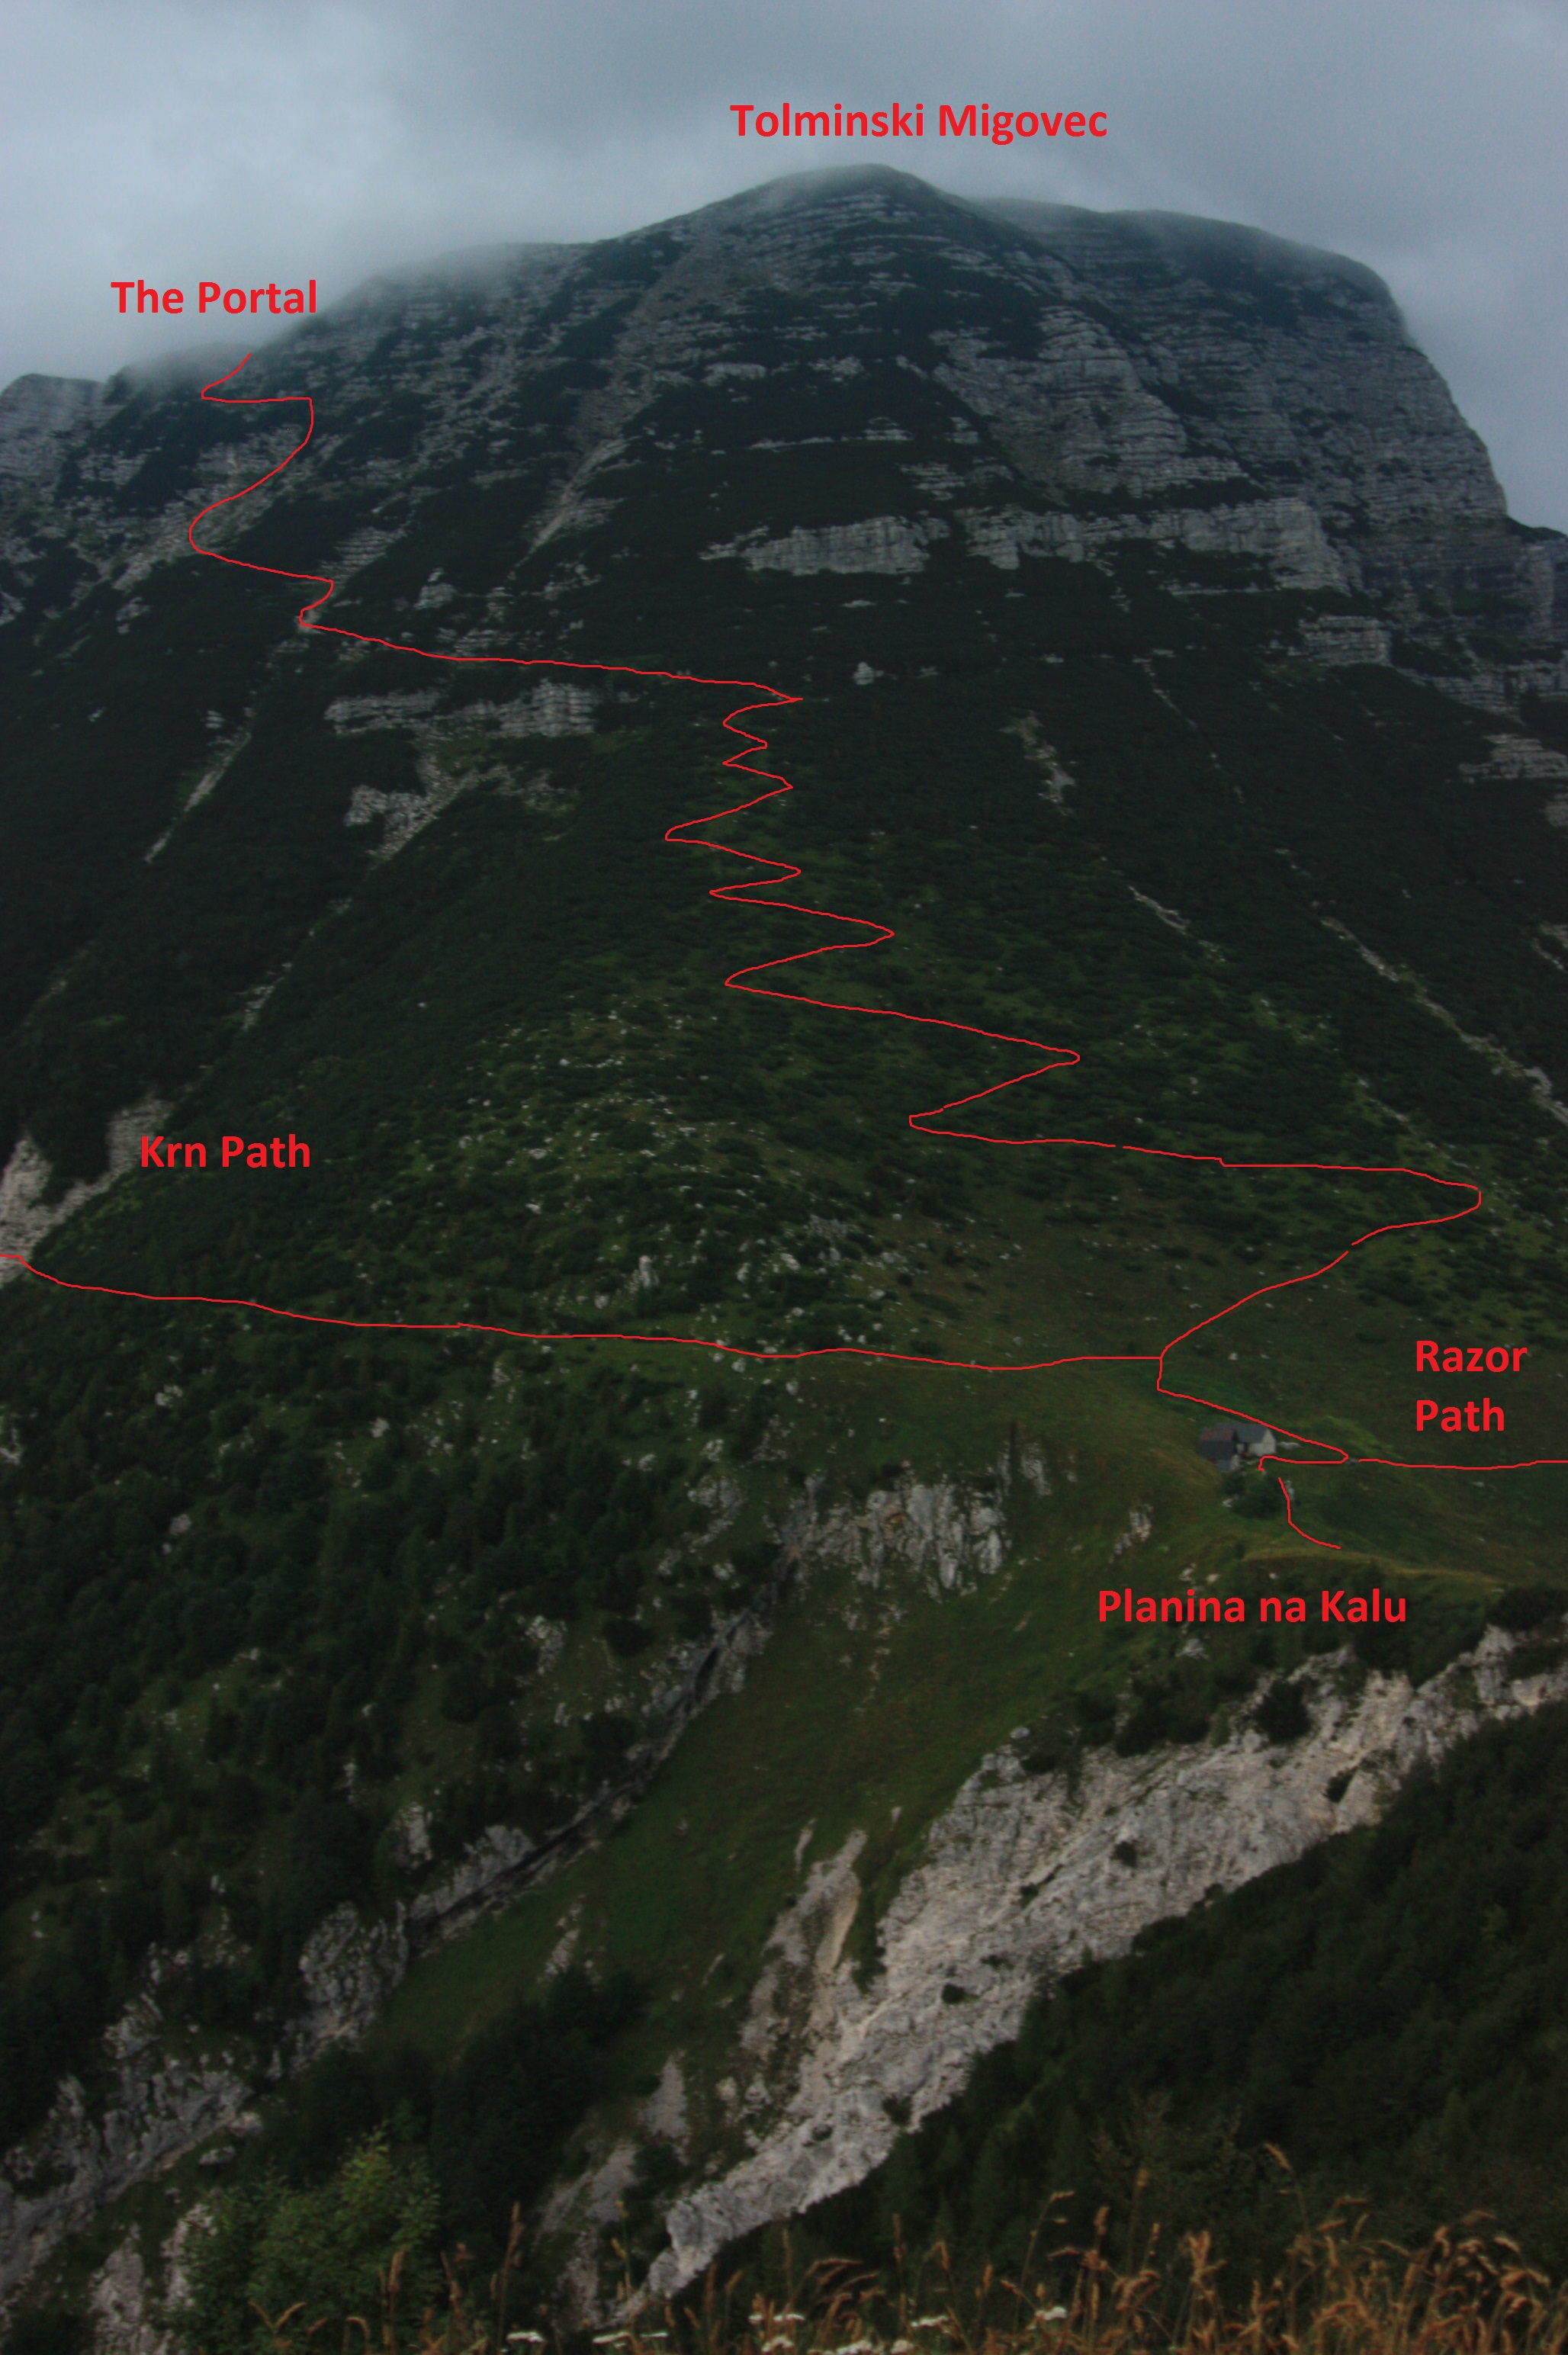
\includegraphics[width=\linewidth, trim ={0 0 0 200pt},clip]{images/2013/welcome-2013/gergely_mig-path.jpg} \caption{The face of \protect\passage{Tolminski Migovec} from nearby \protect\passage{Grusnica}--- Gergely Ambrus}
\end{pagefigure}
